\ifthenelse{\equal{\Langue}{FR}}{
\chapter{Hacheur 4 quadrants utilisé en traction ferroviaire}
}{
\chapter{4-quadrant chopper used in railway traction}
}

% Sources : https://www.techniques-ingenieur.fr/base-documentaire/ingenierie-des-transports-th14/materiel-roulant-ferroviaire-42630210/tramways-c4442/performances-en-traction-et-en-freinage-c4442niv10003.html

%%%%%% Introduction %%%%%%%

\ifthenelse{\equal{\Langue}{FR}}{
\textit{La structure réversible de ce type de hacheur permet d'envisager son utilisation pour le pilotage de machines à courant continu en traction, là où la réversibilité est la plus intéressante à exploiter. Il est utilisé pour toutes les gammes de puissance, l'exemple donné ici étant celui d'un tramway.}

Le tramway est modélisé par une ``voiture'' motorisée par une machine à courant continu, elle-même pilotée par un hacheur réversible alimenté par une source continue parfaite (de type caténaire). Le schéma simplifié du dispositif est représenté sur la figure suivante et correspond aux grandeurs décrites ci-dessous.
}{
\textit{The reversible structure of this type of chopper allows for its use in controlling direct current machines in traction, where reversibility is most interesting to exploit. It is used for all power ranges, with the example given here being that of a tramway.}

The tramway is modeled by a ``car'' powered by a DC machine, itself controlled by a reversible chopper powered by a perfect reversible DC source (catenary type). The simplified diagram of the device is shown in the following figure and corresponds to the described quantities.
}

\begin{figure}[H]
\centering
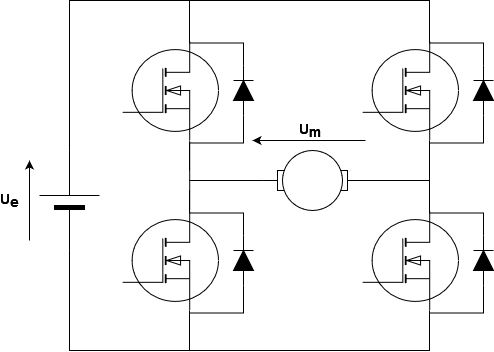
\includegraphics[width=0.55\linewidth]{TD_H4Q/fig/H4Q.png}
\caption{4 Quadrant chopper}
\end{figure}

\ifthenelse{\equal{\Langue}{FR}}{
Le hacheur est alimenté par une source de tension constante de valeur $U_E = 1500 V$. Il est constitué de deux bras de pont indépendants commandés à fréquence fixe $F_d = 2 kHz$. On note les rapports cycliques suivants: $\alpha_1$ pour $T_{11}$ et $\alpha_2$ pour $T_{21}$, la commande de chaque bras étant de type complémentaire. On suppose bien sûr les composants parfaits, diodes et transistors. Entre les deux bras de pont, on maintient la relation de commande suivante: $\alpha_1 + \alpha_2 = 1$.

Le moteur à courant continu est modélisé classiquement par sa f.e.m. $E$, sa résistance d'induit $R$ et son inductance d'induit $L$; son excitation est maintenue constante par un autre dispositif non étudié. La constante de couple (égale à la constante de f.e.m.) est notée $k_\varphi$ et les valeurs numériques sont les suivantes:

$R = 0.2 \Omega$; $L = 25 mH$; $k_\varphi = 7.64 Nm/A$; vitesse nominale $N_n = 1500\text{ tr/min}$.

La voiture du tramway constitue la charge mécanique et présente, vis-à-vis de l'arbre moteur, un moment d'inertie $J = 200 kg.m^2$. En fonction du trajet, elle `` ramène'' également sur cet arbre moteur un couple résistant noté $C_v$.
}{
The chopper is powered by a constant voltage source with a value of $U_E = 1500 V$. It consists of two independent bridge arms controlled at a fixed frequency of $F_d = 2 kHz$. The duty cycles are denoted as follows: $\alpha_1$ for $T_{11}$ and $\alpha_2$ for $T_{21}$, with the control of each arm being complementary. We assume perfect components, diodes, and transistors. Between the two bridge arms, the following control relationship is maintained: $\alpha_1 + \alpha_2 = 1$.

The direct current motor is conventionally modeled by its electromotive force (EMF) $E$, its armature resistance $R$, and its armature inductance $L$; its excitation is kept constant by another device not studied here. The torque constant (equal to the EMF constant) is denoted as $k_\varphi$, and the numerical values are as follows:

$R = 0.2 \Omega$; $L = 25 mH$; $k_\varphi = 7.64 Nm/A$; nominal speed $N_n = 1500 rpm$.

The tramway car constitutes the mechanical load and presents, with respect to the motor shaft, a moment of inertia $J = 200 kg.m^2$. Depending on the trajectory, it also ``returns'' to this motor shaft a resisting torque denoted as $C_v$.
}

%%%%%% Partie 1 %%%%%%%
\begin{enumerate}

\ifthenelse{\equal{\Langue}{FR}}{
\item \textbf{Commande complémentaire totale}
}{
\item \textbf{Total complementary control}
}

\begin{enumerate}

\ifthenelse{\equal{\Langue}{FR}}{
\item Représenter rapidement l'allure de la tension moteur $u_m(t)$ pour un rapport cyclique $\alpha_1$ quelconque, inférieur à $0.5$ puis supérieur à $0.5$.
}{
\item Quickly represent the shape of the motor voltage $u_m(t)$ for any duty cycle $\alpha_1$, first less than $0.5$ and then greater than $0.5$.
}

\ifthenelse{\equal{\SuCorr}{CO}}{
\begin{figure}[H]
\begin{minipage}[b]{0.45\textwidth}
    \centering \underline{$\alpha < 0.5$}
\end{minipage}
\hfill
\begin{minipage}[b]{0.45\textwidth}
    \centering \underline{$\alpha > 0.5$}
\end{minipage}
\vfill
\begin{minipage}[b]{0.45\textwidth}
    \centering
    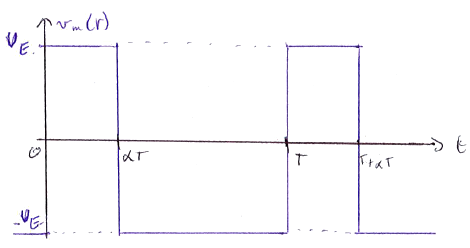
\includegraphics[width=\textwidth]{TD_H4Q/fig/H4Q_1.png}
\end{minipage}
\hfill
\begin{minipage}[b]{0.45\textwidth}
    \centering
    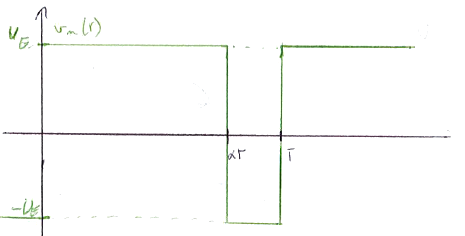
\includegraphics[width=\textwidth]{TD_H4Q/fig/H4Q_2.png}
    \end{minipage}
\end{figure}
}

\ifthenelse{\equal{\Langue}{FR}}{
\item Calculer la valeur moyenne de cette tension, notée $U_m$, en fonction de $\alpha_1$.
}{
\item Calculate the average value of this voltage, denoted as $U_m$, as a function of $\alpha_1$.
}

\ifthenelse{\equal{\SuCorr}{CO}}{
\[U_m = <u_m(t)> = \alpha_1 U_E  - (1-\alpha_1) U_E  = U_E (2\alpha_1 - 1)\]
}

\end{enumerate}
%%%%%% Partie 2 %%%%%%%
\ifthenelse{\equal{\Langue}{FR}}{
\item\textbf{Description fonctionnelle}

On néglige dans cette partie l'ondulation du courant dans le moteur. De plus, un asservissement de courant supposé très rapide devant les constantes de temps mécaniques permet d'imposer la valeur souhaitée au courant d'induit du moteur, celle-ci étant notée $I_M$, constante.
}{
\item \textbf{Functional description}

In this part, we neglect the current ripple in the motor. In addition, a very fast current control compared to the mechanical time constants allows us to impose the desired value on the motor armature current, denoted as $I_M$, which is constant.
}
\begin{enumerate}

\ifthenelse{\equal{\Langue}{FR}}{
\item Exprimer en fonction de $\alpha_1$, $U_E$ et $I_M$, les valeurs moyennes (à la fréquence de découpage $F_d$) de la tension aux bornes de l'induit moteur, notée $U_M$ et du courant absorbé par le hacheur à la source, noté $I_E$.
}{
\item Express the average values (at the switching frequency $F_d$) of the voltage across the motor armature, denoted as $U_M$, and the current drawn by the chopper from the source, denoted as $I_E$, as functions of $\alpha_1$, $U_E$, and $I_M$.
}

\ifthenelse{\equal{\SuCorr}{CO}}{
\[U_m = (2\alpha_1-1)U_E\]

\[V_{DC} \ I_E = U_m I_m \Rightarrow I_E = (2\alpha_1-1)I_m\]
}

\ifthenelse{\equal{\Langue}{FR}}{
\item Le tramway s'arrête en côte (pente montante). Le poids de la voiture exerce alors un couple sur l'arbre moteur de valeur: $C_v$ de $382 Nm$. Quel est le rapport cyclique $\alpha_{10}$ nécessaire pour maintenir le tramway à l'arrêt? Que vaut alors le courant $I_{E0}$ prélevé à la source d'alimentation (toujours en valeur moyenne)?
}{
\item The tramway stops on an \textbf{uphill} slope. The weight of the car then exerts a torque on the motor shaft with a value of $C_v = 382 Nm$. What is the duty cycle $\alpha_{10}$ required to keep the tramway at a standstill? What is the current $I_{E0}$ drawn from the power supply (still in average value)?
}

\ifthenelse{\equal{\SuCorr}{CO}}{
\ifthenelse{\equal{\Langue}{FR}}{
Attention dans cette partie, $C_v = -382 \text{ Nm}$ car le train est en montée donc le couple est négatif.
}{
Be carefull in this part, $C_v = -382 \text{ Nm}$ because the train is going uphill so torque is negative.
}

$v_m(t) = R i_m(t) + L \frac{di_m(t)}{dt} + E$
        
$V_m = <v_m(t)> = R <i_m(t)> + L <\frac{di_m(t)}{dt}> + <E>$
\begin{itemize}
    \item $<E> = 0$ \ifthenelse{\equal{\Langue}{FR}}{car}{because} $\Omega = 0$
    \item $<\frac{di_m(t)}{dt}> = 0 $ \ifthenelse{\equal{\Langue}{FR}}{car}{because} $i_m(t)$ \ifthenelse{\equal{\Langue}{FR}}{est périodique}{is periodic}
\end{itemize}
\begin{equation}
    \Rightarrow V_m = (2\alpha -1) U_E = R I_m
\end{equation}
$J \dfrac{d\Omega}{dt} = C_m + C_v = k_\Phi i_m + C_v \Rightarrow I_M = -\dfrac{C_v}{k_\Phi}$

(1.1) $\Rightarrow V_m = - R \dfrac{C_v}{k_\Phi} \Rightarrow \alpha_{10} = \left(1 + \dfrac{- C_v R}{k_\Phi U_E} \right) \dfrac{1}{2} \approx 0.503$

$I_{E0} = (2\alpha_{10} - 1) I_m = (2 \alpha_{10} - 1) \dfrac{-C_v}{k_\Phi} = \dfrac{R C_v^2}{k_\Phi^2 U_E} \approx 0.33 \text{ A}$

}

\ifthenelse{\equal{\Langue}{FR}}{
\item Le tramway démarre à plat (on néglige le couple résistant) avec une accélération constante de $5 rad/s^2$ jusqu'à atteindre la vitesse de rotation nominale du moteur. 
}{
\item The tramway starts on a level track (neglecting the resisting torque) with a constant acceleration of $5 rad/s^2$ until it reaches the nominal motor speed.

}
\begin{enumerate}

\ifthenelse{\equal{\Langue}{FR}}{
\item Que vaut alors le courant moteur $I_m$?
}{
\item What is the current $I_m$ in the motor?
}

\ifthenelse{\equal{\SuCorr}{CO}}{
\ifthenelse{\equal{\Langue}{FR}}{Pas de couple résistant}{No resistive torque}: $C_v = 0$
        
$J \dfrac{d\Omega}{dt} = C_m + C_v = k_\Phi I_m \Rightarrow I_m = \dfrac{J}{k_\Phi} \dfrac{d\Omega}{dt} = 130 \text{ A}$
}


\ifthenelse{\equal{\Langue}{FR}}{
\item Tracer l'évolution du rapport cyclique $\alpha_{1}$ lors de cette phase d'accélération.
}{
\item Plot the variation of the duty cycle $\alpha_{1}$ during this acceleration phase.
}

\ifthenelse{\equal{\SuCorr}{CO}}{
$V_m = (2\alpha -1) U_E = R I_m + L \dfrac{di_m}{dt} + E$
\begin{itemize}
    \item $E = K_\Phi \Omega = k_\Phi \dfrac{d\Omega}{dt} t$ \ifthenelse{\equal{\Langue}{FR}}{car}{because} $\dfrac{d\Omega}{dt} = constant$ \ifthenelse{\equal{\Langue}{FR}}{et}{and} $\Omega (t=0)=0$
    \item $\dfrac{di_m}{dt} = 0$ ($i_m$ constant)
\end{itemize}
$(2\alpha -1) U_E = R I_m + k_\Phi \left(\dfrac{d\Omega}{dt}\right) t$

$\Rightarrow \alpha (t) = \dfrac{1}{2}\left(\dfrac{R I_m}{U_E} + \dfrac{k_\Phi}{U_E} \left(\dfrac{d\Omega}{dt}\right) t + 1\right)$
}

\ifthenelse{\equal{\Langue}{FR}}{
\item Tracer l'évolution du courant $I_E$ prélevé à la source lors de cette phase d'accélération.
}{
\item Plot the variation of the current $I_E$ drawn from the power supply during this acceleration phase.
}

\ifthenelse{\equal{\SuCorr}{CO}}{
$I_E = (2\alpha_1-1)I_m$ et $\alpha_1(t)$

$\Rightarrow I_E(t) = \left(\dfrac{R I_m}{U_E} + \dfrac{k_\Phi}{U_E} \left(\dfrac{d\Omega}{dt}\right) t\right) I_m$
}

\ifthenelse{\equal{\Langue}{FR}}{
\item Calculer la durée d'accélération $\Delta t_a$.
}{
\item Calculate the acceleration time $\Delta t_a$.
}

\ifthenelse{\equal{\SuCorr}{CO}}{
$\left(\dfrac{d\Omega}{dt}\right) \Delta t_a = \Omega_n \Rightarrow \Delta t_a = \dfrac{\Omega_n}{\left(\dfrac{d\Omega}{dt}\right)} = 31 \text{ s}$
}

\end{enumerate}

\ifthenelse{\equal{\Langue}{FR}}{
\item Le tramway effectue un trajet \textbf{en descente} à vitesse constante, le moteur tournant à sa vitesse nominale. Le poids exerce un couple $C_v$ de $382 Nm$. Que vaut le courant $I_{Ed}$ prélevé à la source d'alimentation? Quel est alors la valeur du rapport cyclique $\alpha_{1d}$ permettant ce fonctionnement à vitesse constante?
}{
\item The tramway travels on a \textbf{downhill} trajectory at a constant speed, with the motor running at its nominal speed. The weight exerts a torque $C_v = 382 Nm$. What is the current $I_{Ed}$ drawn from the power supply? What is the value of the duty cycle $\alpha_{1d}$ that allows for this constant speed operation?
}

\ifthenelse{\equal{\SuCorr}{CO}}{
\ifthenelse{\equal{\Langue}{FR}}{
Attention dans cette partie, $C_v = 382 \text{ Nm}$ car le train est en descente donc le couple est positif.
}{
Be carefull in this part, $C_v = 382 \text{ Nm}$ because the train is going downhill so torque is positive.
}
\begin{itemize}
\item $J \dfrac{d\Omega}{dt} = C_m + C_v = k_\Phi i_m + C_v$
\item $\dfrac{d\Omega}{dt} = 0$ \ifthenelse{\equal{\Langue}{FR}}{car}{because} $\Omega = constant \Rightarrow i_m = \dfrac{-C_v}{k_\Phi} = -50 \text{ A}$
\end{itemize}

$U_E I_{Ed} = V_m I_m \Rightarrow I_{Ed}= \dfrac{V_m I_m}{U_E} = \dfrac{R I_m^2 + k_\Phi \Omega I_m}{U_E} = -39.7 \text{ A}$

}

\ifthenelse{\equal{\Langue}{FR}}{
\item Freinage d'urgence en descente: lors du fonctionnement précédent (1.3), le conducteur demande un freinage d'urgence caractérisé par l'asservissement du courant d'induit à la valeur maximale tolérable par le hacheur et la machine, $I_{\max} = 250 A$. On suppose que ce courant est imposé de façon quasi instantanée et reste présent lors de la phase de décélération, le couple lié au poids de la voiture étant toujours inchangé, égal à $382 Nm$.
}{
\item Emergency braking downhill: during the previous operation (1.3), the driver requests emergency braking characterized by controlling the armature current to the maximum value tolerable by the chopper and the machine, $I_{\max} = 250 A$. We assume that this current is imposed quasi-instantaneously and remains present during the deceleration phase, with the torque related to the weight of the car remaining unchanged at $382 Nm$.
}

\begin{enumerate}

\ifthenelse{\equal{\Langue}{FR}}{
\item Calculer et représenter l'évolution temporelle de la vitesse de rotation du moteur $\Omega(t)$, image de la vitesse du tramway.
}{
\item Calculate and represent the time evolution of the motor speed $\Omega(t)$, which represents the tramway speed.
}

\ifthenelse{\equal{\SuCorr}{CO}}{
$J \dfrac{d\Omega}{dt} = C_m + C_v = k_\Phi i_m + C_v$
            
$I_m = - I_{\max}$.\ifthenelse{\equal{\Langue}{FR}}{Le courant est négatif pour freiner.}{The current is negative to break.}

$J \dfrac{d\Omega}{dt} = - k_\Phi I_{\max} + C_v = constant \Rightarrow \Omega = \dfrac{C_v - k_\Phi I_{\max}}{J} t + \Omega_n$

\begin{figure}[H]
    \centering
    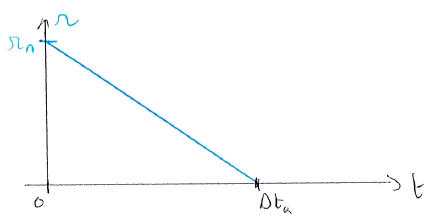
\includegraphics[width=0.6\linewidth]{TD_H4Q/fig/H4Q_Omega.png}
\end{figure}
}

\ifthenelse{\equal{\Langue}{FR}}{
\item Calculer la durée de ralentissement jusqu'à l'arrêt, notée $\Delta t_a$.
}{
\item Calculate the deceleration time until stop, denoted as $\Delta t_a$.
}

\ifthenelse{\equal{\SuCorr}{CO}}{
$\Omega (t=\Delta t_a)= 0 \Rightarrow \dfrac{C_v - k_\Phi I_{\max}}{J} \Delta t_a = - \Omega_n$ 

$\Rightarrow \Delta t_a = \dfrac{\Omega_n J}{k_\Phi I_{\max} - C_v} = 21 \text{ s}$
}

\ifthenelse{\equal{\Langue}{FR}}{
\item Déterminer lors de cette phase l'évolution du rapport cyclique $\alpha_1(t)$ en précisant notamment sa valeur au début du freinage et juste avant l'arrêt du véhicule.
}{
\item Determine the evolution of the duty cycle $\alpha_1(t)$ during this phase, specifying its value at the beginning of braking and just before the vehicle comes to a stop.
}

\ifthenelse{\equal{\SuCorr}{CO}}{
$V_m = (2\alpha -1) U_E = R I_m + E = - R I_{\max} + k_\Phi \Omega$
            
$\Rightarrow \alpha = \dfrac{1}{2} + \dfrac{k_\Phi \Omega - R I_{\max}}{2 U_E}$

\begin{itemize}
    \item \ifthenelse{\equal{\Langue}{FR}}{Début du freinage:}{Start Breaking} $\Omega = \Omega_n \Rightarrow \alpha = 0.88$
    \item \ifthenelse{\equal{\Langue}{FR}}{Avant l'arrêt:}{Before Stop} $\Omega = 0 \Rightarrow \alpha = 0.48$
\end{itemize}
}


\ifthenelse{\equal{\Langue}{FR}}{
\item Calculer l'énergie totale $E_C$ restituée à la source lors de ce freinage.
}{
\item Calculate the total energy $E_C$ returned to the source during this braking operation.
}

\ifthenelse{\equal{\SuCorr}{CO}}{
$\begin{aligned}
    E_C &= \int_{0}^{\Delta t_a} -V_m I_m dt = \int_{0}^{\Delta t_a} \left(-R I_{\max}^2 + k_\Phi \Omega I_{\max} \right) dt \\
    &= -R I_{\max}^2 \Delta t_a + \int_{0}^{\Delta t_a} k_\Phi I_{\max} \left(\dfrac{C_v - k_\Phi I_{\max}}{J} t + \Omega_n \right) dt \\
    & \cdots \\
    &= \dfrac{\Omega_n J}{k_\Phi I_{\max} - C_v} \left( \dfrac{k_\Phi I_{\max} \Omega_n}{2} - R I_{\max}^2 \right) = 2.8 \text{ MJ}
\end{aligned}$
}

\end{enumerate}

\ifthenelse{\equal{\Langue}{FR}}{
\item Représenter les quadrants de fonctionnement du hacheur utilisés lors des différentes phases de fonctionnement du tramway.
}{
\item Represent the operating quadrants of the chopper used during the different phases of the tramway operation.
}

\ifthenelse{\equal{\SuCorr}{CO}}{
\begin{figure}[H]
    \centering
    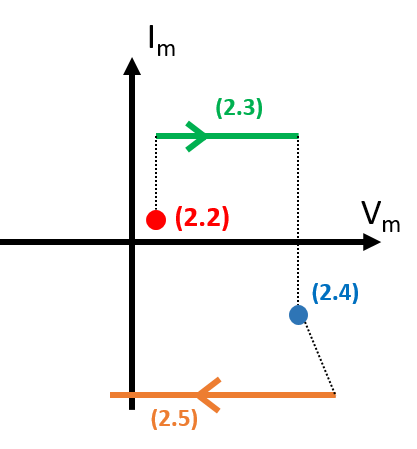
\includegraphics[width=0.6\linewidth]{TD_H4Q/fig/H4Q_quadrant.png}
\end{figure}
}

\end{enumerate}

% \newpage
% \item \textbf{Commande complémentaire décalée du hacheur}

% On se propose ici de changer la commande des interrupteurs. Elle est réalisée suivant le schéma de la figure suivante. Pour chaque ``bras de pont'', la commande est toujours complémentaire de fréquence $F_d$ (on suppose que les commutations sont instantanées). Pour réaliser les modulations du rapport cyclique, on réalise la comparaison entre une modulatrice ($M_1$ ou $M_2$) et la tension image du rapport cyclique $\alpha$, notée $v_{alpha}$. On suppose que la sortie de ces comparateur est un signal binaire permettant de
% commander les interrupteurs.

% \begin{figure}[H]
% \centering
% 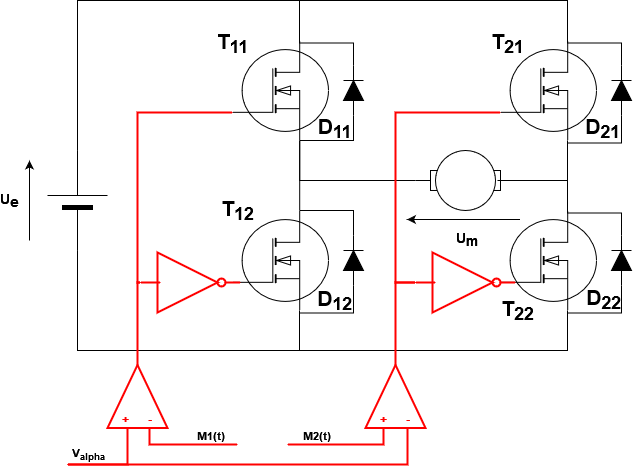
\includegraphics[width=0.6\linewidth]{TD_H4Q/fig/H4Q_decale.png}
% \caption{Shifted control of a 4 quadrant chopper}
% \end{figure}

% Les deux modulatrices sont représentées sur la figure suivante : il s'agit de signaux triangulaires en opposition de phase et d'amplitude $1 V$. Le signal $v_{alpha}$ est lui même d'amplitude maximale $1 V$, son amplitude réelle étant proportionnelle au rapport cyclique $\alpha$.

% \begin{enumerate}
% \item Pour $\alpha = 0.8$, représenter l'allure des fonctions de commutation $f_1(t)$ et $f_2(t)$ ainsi que la tension $u_m(t)$ aux bornes du moteur.
% \item Quelle est la fréquence de ce signal $u_m$ ? Quel est son ``rapport cyclique'', noté $\beta$ ?
% \item Pour $\alpha = 0.2$, représenter l'allure des fonctions de commutation $f_1(t)$ et $f_2(t)$ ainsi que la tension $u_m(t)$ aux bornes du moteur.
% \item Lorsque $\alpha$ est compris entre 0.5 et 1 et en négligeant la résistance $R$, déterminer l'ondulation $\Delta I_M$ du courant moteur. Quelle est sa valeur maximale $\Delta I_{M max}$?
% \item Quel est l'intérêt de cette commande par rapport à la commande complémentaire totale ?
% \end{enumerate}


% \newpage
% \begin{figure}[H]
% \centering
% 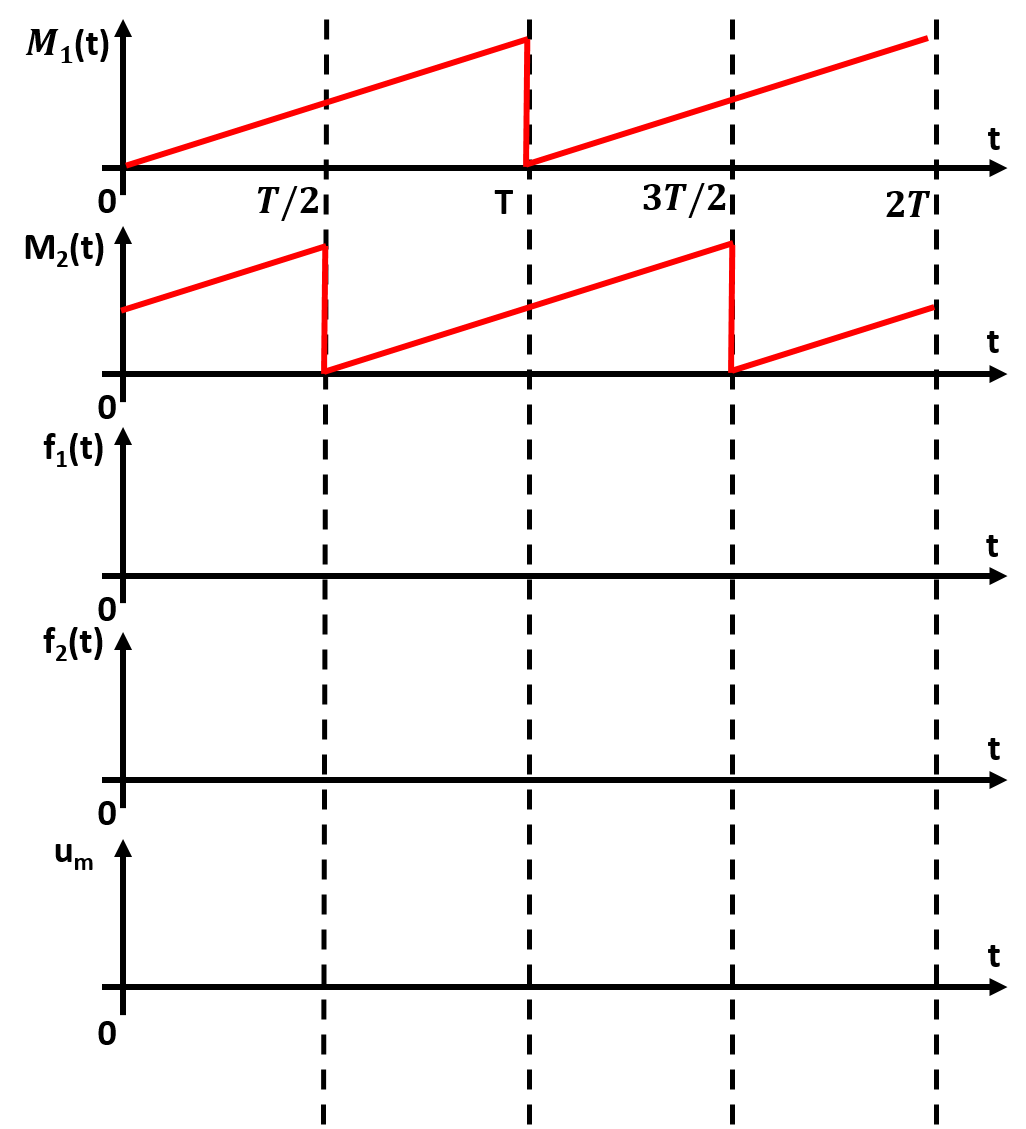
\includegraphics[width=\linewidth]{TD_H4Q/fig/answer.png}
% \caption{Shifted control of a 4 quadrant chopper}
% \end{figure}

%\newpage
%\item \textbf{Commande indépendante}
%
%On se propose ici de changer la commande des interrupteurs. Les transistors $T_{11}$ et $T_{12}$ sont toujours commandés de manière complémentaire avec le même signal que précédemment. les transistors $T_{21}$ et $T_{22}$ sont cette fois-ci commandés en fonction du signe de la tension de sortie souhaité : pour une tension $U_m$ positive, $T_{22}$ est fermé et $T_{21}$ est ouvert, et pour une tension $U_m$ négative, $T_{22}$ est ouvert et $T_{21}$ est fermé.
%
%\begin{figure}[H]
%\centering
%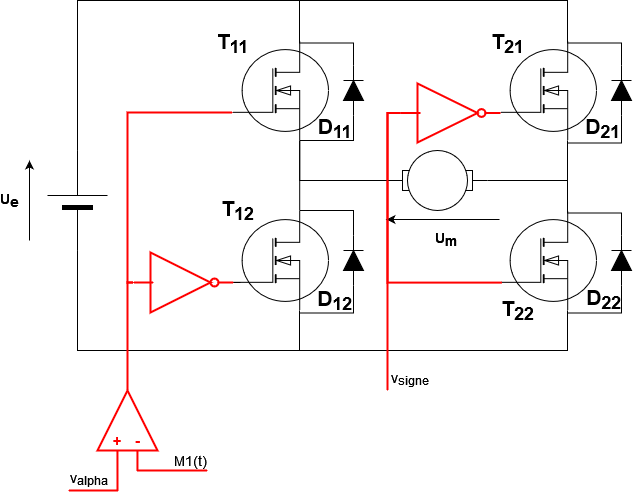
\includegraphics[width=0.6\linewidth]{TD_H4Q/fig/H4Q_indep.png}
%\caption{Independant control 4 quadrant chopper}
%\end{figure}
%
%\begin{enumerate}
%\item Représenter l'allure de $u_m(t)$ pour $\alpha=0.25$ et $v_{signe}=1$
%
%\item En déduire la relation entre la valeur moyenne de $u_m(t)$ et $\alpha$ lorsque $v_{signe}=1$
%
%\item Représenter l'allure de $u_m(t)$ pour $\alpha=0.25$ et $v_{signe}=0$
%
%\item En déduire la relation entre la valeur moyenne de $u_m(t)$ et $\alpha$ lorsque $v_{signe}=0$
%
%\item Conclure sur les avantages et inconvénients des différentes commandes
%\end{enumerate}
%
%\begin{figure}[H]
%\centering
%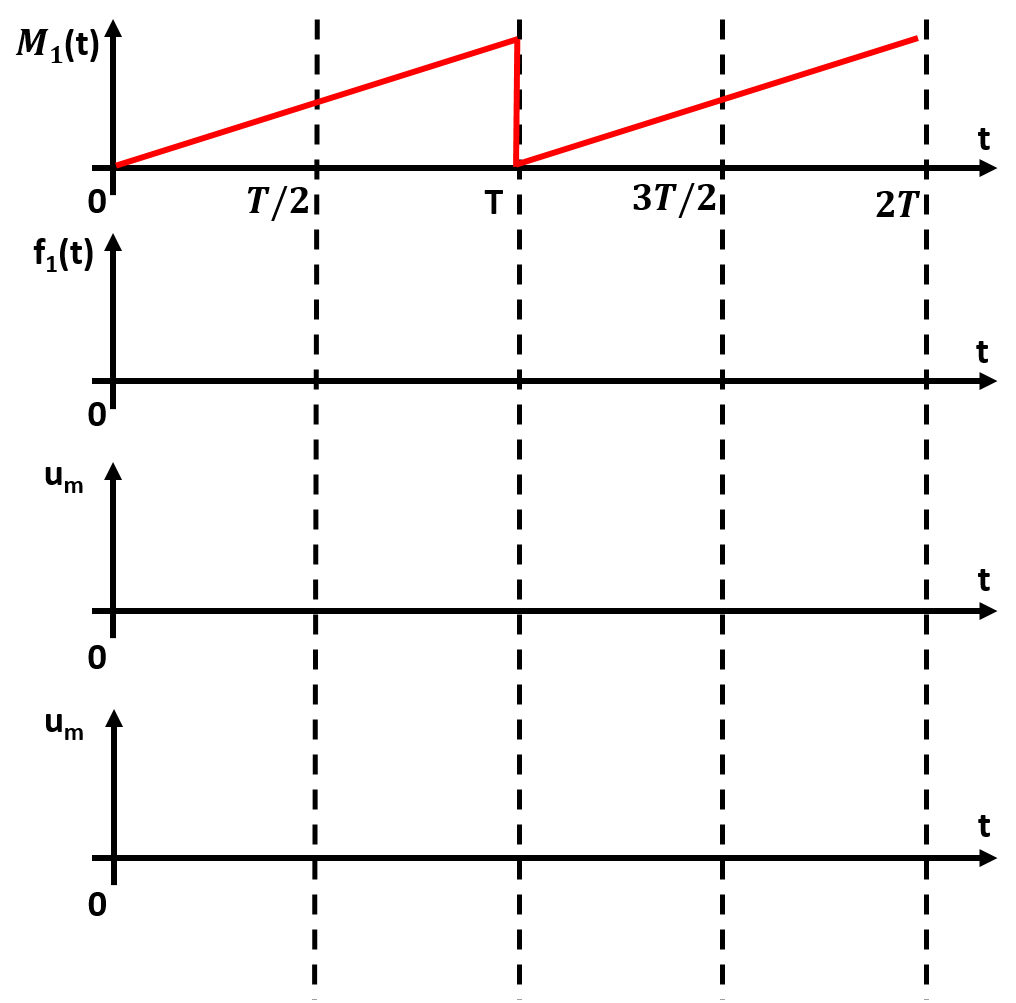
\includegraphics[width=\linewidth]{TD_H4Q/fig/answer2.png}
%%\caption{Shifted control of a 4 quadrant chopper}
%\end{figure}

\end{enumerate}


